% ============================================================
%  PRESENTACIÓN: Artículo Científico y Ética Académica
% ============================================================
\documentclass[aspectratio=169, 12pt]{beamer}

\usepackage{fontspec}
\usepackage{tikz}
\usepackage{xcolor}
\usepackage{graphicx}
\usepackage{microtype}
\usepackage{tcolorbox}
\usepackage{calc}
\usepackage{ragged2e}

\usetikzlibrary{positioning, shapes.geometric, fadings}

% ── Fonts ────────────────────────────────────────────────────
\setmainfont{Times New Roman}
\setsansfont{Arial}
\setmonofont{Consolas}[Scale=MatchLowercase]

% ── Colour palette ───────────────────────────────────────────
\definecolor{Obsidian}{HTML}{0D0D0D}
\definecolor{Charcoal}{HTML}{1A1A1A}
\definecolor{Slate}{HTML}{2C2C2C}
\definecolor{Ember}{HTML}{E8643A}
\definecolor{Gold}{HTML}{C49A3C}
\definecolor{Smoke}{HTML}{8A8A8A}
\definecolor{Cloud}{HTML}{D6D6D6}
\definecolor{OffWhite}{HTML}{F5F5F5}
\definecolor{SteelBlue}{HTML}{5B8FA8}

% ── Base Beamer settings ─────────────────────────────────────
\usetheme{default}
\usecolortheme{default}
\setbeamertemplate{navigation symbols}{}
\setbeamertemplate{footline}{}

\setbeamercolor{background canvas}{bg=Obsidian}
\setbeamercolor{normal text}{fg=Cloud}
\setbeamercolor{frametitle}{fg=OffWhite}
\setbeamertemplate{frametitle}{\vspace{8pt}{\color{OffWhite}\rmfamily\bfseries\Large\insertframetitle}\ifx\insertframesubtitle\empty\else\\[2pt]{\color{Smoke}\sffamily\small\insertframesubtitle}\fi\vspace{4pt}\emberrule}
\setbeamerfont{normal text}{family=\sffamily}

% Remove default beamer chrome
\setbeamertemplate{headline}{}
\setbeamertemplate{footline}{}
\setbeamertemplate{sidebar left}{}
\setbeamertemplate{sidebar right}{}

% ── Reusable helpers ─────────────────────────────────────────

% Ember accent rule (full-width top bar variant)
\newcommand{\emberrule}{%
  
\begin{tikzpicture}
    \fill[Ember] (0,0) rectangle (\textwidth, 1.5pt);
  \end{tikzpicture}\vspace{4pt}%
}

% Chip / label badge
\newcommand{\chip}[2][Ember]{%
  \tcbox[on line, colback=#1, colframe=#1, arc=1pt,
         boxsep=1pt, left=4pt, right=4pt, top=1.5pt, bottom=1.5pt,
         fontupper=\sffamily\tiny\bfseries\color{OffWhite}\MakeUppercase]{#2}%
}

% Stat card (number + label)
\newcommand{\statcard}[3][Ember]{%
  \begin{tcolorbox}[
    colback=Slate, colframe=#1, arc=0pt,
    leftrule=4pt, rightrule=0pt, toprule=0pt, bottomrule=0pt,
    left=6pt, right=6pt, top=6pt, bottom=6pt,
  ]
    {\color{OffWhite}\rmfamily\bfseries\fontsize{26}{28}\selectfont #2}\\[3pt]
    {\color{Smoke}\sffamily\fontsize{6.5}{6.5}\selectfont\MakeUppercase{#3}}
  \end{tcolorbox}%
}

% Image placeholder (replace \imageph with \includegraphics in real use)
\newcommand{\imageph}[2][5cm]{%
  \begin{tikzpicture}
    \fill[Charcoal] (0,0) rectangle (\linewidth,#1);
    \node[text=Slate!60!Charcoal, font=\sffamily\tiny\itshape]
      at (0.5\linewidth, 0.5*#1) {#2};
  \end{tikzpicture}%
}

% Icon illustrations (TikZ) to avoid external images
\newcommand{\bookicon}[1][2cm]{%
  \begin{tikzpicture}[scale=1, baseline={(current bounding box.center)}]
    \fill[OffWhite] (0,0) rectangle (#1,0.8#1);
    \draw[black,line width=0.8pt] (0,0) rectangle (#1,0.8#1);
    \fill[Slate] (0.05#1,0.1#1) rectangle (0.25#1,0.7#1);
    \draw (0.03#1,0.1#1) -- (0.03#1,0.7#1);
    \draw (0.27#1,0.1#1) -- (0.27#1,0.7#1);
    \node[anchor=north west, font=\sffamily\tiny] at (0.3#1,0.7#1) {ARTÍCULO};
  \end{tikzpicture}%
}

\newcommand{\mapicon}[1][2cm]{%
  \begin{tikzpicture}[scale=1, baseline={(current bounding box.center)}]
    \fill[OffWhite] (0,0) rectangle (#1,0.8#1);
    \draw[black,line width=0.8pt] (0,0) rectangle (#1,0.8#1);
    \draw[Slate,line width=0.9pt] (0.08#1,0.6#1) -- (0.3#1,0.72#1) -- (0.55#1,0.45#1) -- (0.78#1,0.6#1);
    \node[anchor=south, font=\sffamily\tiny, text=Ember] at (0.35#1,0.2#1) {C.R.};
  \end{tikzpicture}%
}

\newcommand{\balanceicon}[1][2cm]{%
  \begin{tikzpicture}[scale=1, baseline={(current bounding box.center)}]
    \draw[black,line width=0.8pt] (0.5,0) -- (0.5,0.8#1);
    \draw[black,line width=0.8pt] (0.2,0.8#1) -- (0.8,0.8#1);
    \draw[black,line width=0.6pt] (0.25,0.8#1) -- (0.5,0.7#1) -- (0.75,0.8#1);
    \draw[black,line width=0.6pt] (0.28,0.52#1) -- (0.31,0.2#1); 
    \draw[black,line width=0.6pt] (0.72,0.52#1) -- (0.69,0.2#1);
    \fill[Ember] (0.22,0.28#1) circle (0.03#1);
    \fill[Ember] (0.68,0.28#1) circle (0.03#1);
  \end{tikzpicture}%
}

% Full-bleed background helper (used inside tikzpicture overlays)
% Usage: \fullbg{color} inside frame with [plain]
\newcommand{\fullbg}[1]{%
  \begin{tikzpicture}[remember picture, overlay]
    \fill[#1] (current page.south west) rectangle (current page.north east);
  \end{tikzpicture}%
}

% ── Footer bar ───────────────────────────────────────────────
\setbeamertemplate{footline}{%
  \begin{tikzpicture}[remember picture, overlay]
    \fill[Charcoal]
      (current page.south west) rectangle
      ([yshift=14pt]current page.south east);
    \node[anchor=west, text=Smoke, font=\sffamily\fontsize{5}{5}\selectfont,
          inner sep=0] at ([xshift=10pt, yshift=7pt]current page.south west)
      {OBSIDIAN \& EMBER TEMPLATE};
    \node[anchor=east, text=Smoke, font=\sffamily\fontsize{5}{5}\selectfont,
          inner sep=0] at ([xshift=-10pt, yshift=7pt]current page.south east)
      {\insertframenumber\,/\,\inserttotalframenumber};
  \end{tikzpicture}%
}

% ============================================================
\begin{document}
% ============================================================

% ── SLIDE 1: Title ───────────────────────────────────────────
{
\setbeamertemplate{footline}{}   % no footer on title
\begin{frame}[plain]
  \begin{tikzpicture}[remember picture, overlay]

    % Left image panel
    \fill[Charcoal]
      (current page.south west) rectangle
      ([xshift=0.52\paperwidth]current page.north west);
    % Ember vertical rule
    \fill[Ember]
      ([xshift=0.52\paperwidth]current page.south west)
      rectangle
      ([xshift=0.525\paperwidth]current page.north west);

    % Image placeholder text
    \begin{scope}
      \clip (current page.south west) rectangle ([xshift=0.52\paperwidth]current page.north west);
      \node[anchor=north west] at (current page.north west) {
        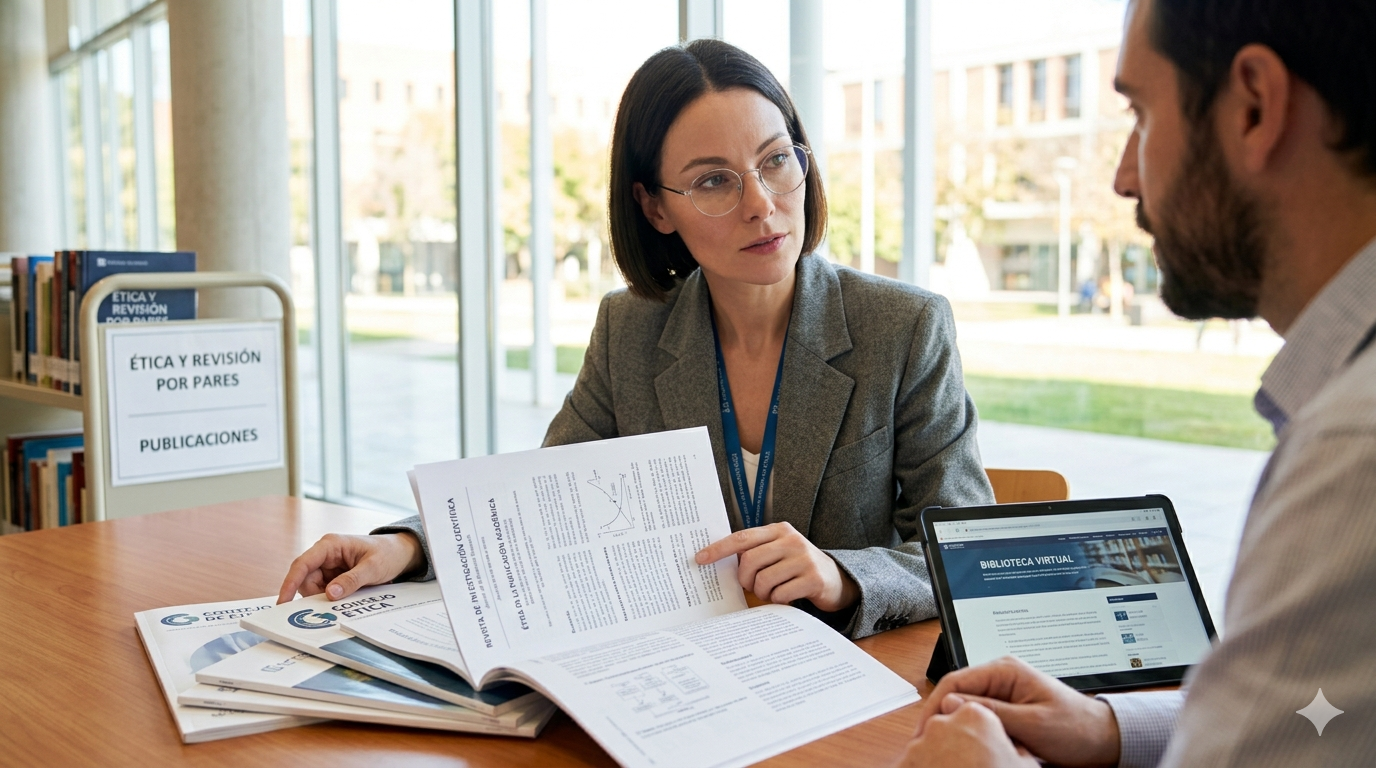
\includegraphics[height=\paperheight,
                        keepaspectratio,
                        trim=500 0 150 0,
                        clip]{imagenes/portada.png}
      };
    \end{scope}

    % Eyebrow label
    \node[anchor=north west,
          text=Gold,
          font=\sffamily\fontsize{7}{7}\selectfont\bfseries,
          inner sep=0,
          xshift=0.55\paperwidth, yshift=-0.10\paperheight]
      at (current page.north west)
      {\MakeUppercase{Tecnológico de Costa Rica}};

    \node[anchor=north west,
          text=Gold,
          font=\sffamily\fontsize{7}{7}\selectfont\bfseries,
          inner sep=0,
          xshift=0.55\paperwidth, yshift=-0.15\paperheight]
      at (current page.north west)
      {\MakeUppercase{Maestría en Ciencias de la Computación}};

    % Big title — word 1
    \node[anchor=north west,
          text=OffWhite,
          font=\rmfamily\fontsize{32}{32}\selectfont\bfseries,
          inner sep=0,
          xshift=0.545\paperwidth, yshift=-0.30\paperheight]
      at (current page.north west) {ARTÍCULO};

    % Big title — word 2 (accent)
    \node[anchor=north west,
          text=Ember,
          font=\rmfamily\fontsize{32}{32}\selectfont\bfseries,
          inner sep=0, text width=0.42\paperwidth,
          xshift=0.545\paperwidth, yshift=-0.40\paperheight]
      at (current page.north west) {CIENTÍFICO};

    % Subtitle
    \node[anchor=north west,
          text=Cloud,
          font=\sffamily\fontsize{9}{13}\selectfont,
          text width=0.39\paperwidth,
          inner sep=0,
          xshift=0.55\paperwidth, yshift=-0.55\paperheight]
      at (current page.north west)
      {\& Ética Académica en Costa Rica};

    % Divider line
    \draw[Slate, line width=0.4pt]
      ([xshift=0.55\paperwidth, yshift=0.18\paperheight]current page.south west)
      -- ([xshift=0.97\paperwidth, yshift=0.18\paperheight]current page.south west);

    % Presenter info
    \node[anchor=west,
          text=Smoke,
          font=\sffamily\fontsize{8}{8}\selectfont,
          inner sep=0,
          xshift=0.55\paperwidth, yshift=0.14\paperheight]
      at (current page.south west)
      {EMMANUEL BARRANTES VARGAS};

  \end{tikzpicture}
\end{frame}
}

% ── SLIDE 2: Contenido ─────────────────────────
\begin{frame}{Contenido}
  \framesubtitle{\space}
  \vspace{-4pt}

  \begin{itemize}
    \item {\bfseries Introducción}
    \item {\bfseries Artículo Científico} 
    \item {\bfseries Ética Académica}   
  \end{itemize}

\end{frame}

\end{document}